\documentclass[12pt,a4paper,openright,twoside]{book}
\usepackage[utf8]{inputenc}
\usepackage{disi-thesis}
\usepackage{code-lstlistings}
\usepackage{notes}
\usepackage{shortcuts}
\usepackage{acronym}

\school{\unibo}
\programme{Corso di Laurea in Ingegneria e Scienze Informatiche}
\title{B-Tree File System per piattaforme IoT}
\author{Leonardo Marcaccio}
\date{\today}
%TODO Vedi se toglier
\subject{Supervisor's course name}

\supervisor{Marco Antonio Boschetti}

\session{I}
\academicyear{2023-2024}

% Definition of acronyms
\acrodef{IoT}{Internet of Thing}
\acrodef{vm}[VM]{Virtual Machine}
\acrodef{FS}{File System}

\mainlinespacing{1.241}

\begin{document}

\frontmatter\frontispiece

\begin{abstract}
    Questa Tesi esplora il processo di studio, progettazione e implementazione di un prototipo di \ac{FS} basato sulla struttura dati B-Tree, sviluppato per la piattaforma IoT IOtto di Onit S.p.A.

    L'obiettivo principale è migliorare l'efficienza nella gestione e nel recupero dei dati, affrontando le problematiche tipiche di un \ac{FS} come la scalabilità e l'ottimizzazione delle risorse.

    Il lavoro comprende un'analisi dello stato dell'arte sui moderni \ac{FS}, con particolare attenzione alla loro interazione con i sistemi IoT. Viene approfondito il principio di funzionamento del B-Tree, dimostrando come questa struttura dati possa essere sfruttata per realizzare una struttura performante e affidabile.

    Inoltre, vengono descritte le fasi di progettazione e implementazione, evidenziando le soluzioni adottate per adattare il prototipo alle esigenze specifiche della piattaforma IOtto.

    I risultati preliminari mostrano che il prototipo proposto garantisce significativi miglioramenti in termini di velocità di accesso ai dati e utilizzo delle risorse rispetto alle alternative tradizionali.
\end{abstract}

\begin{dedication} % this is optional
Optional. Max a few lines.
\end{dedication}

%----------------------------------------------------------------------------------------
\tableofcontents
\listoffigures     % (optional) comment if empty
\lstlistoflistings % (optional) comment if empty
%----------------------------------------------------------------------------------------

\mainmatter

%----------------------------------------------------------------------------------------
\chapter{Introduction}
\label{chap:introduction}
%----------------------------------------------------------------------------------------

    \section{Background}
    \label{sec:background}

        \subsection{Onit}
        \subsection{IOtto}

        AGGIUNGI PRESENTAZIONE DELL'AZIENDA E DEL PRODOTTO

    \section{Descrizione del problema}

        L'attuale \ac{FS} utilizzato dall'applicativo risulta non essere più ottimale nel contesto attuale, data la crescita e la mole dei dati gestiti.
        Risulta dunque necessario trovare un'alternativa che soddisfi le necessità attuali e future, in ambito di scalabilità e ottimizzazione.

    \section{Obiettivi di Tesi}

        L'obbiettivo della Tesi risulta essere quello di realizzare un prototipo di \ac{FS} che sia scalabile, in grado di effettuare rapide letture e scritture, strutturalmente solido e ottimizzato nell'allocazione di spazio.

        In particolare, il lavoro si concentra sulla progettazione e realizzazione di un prototipo alternativo al sistema preesistente, con l'intento non solo di mantenere le prestazioni attuali, ma, ove possibile, di migliorarle.

        \subsection{Domande}
        \label{subsec:Domande}

            \begin{itemize}
                \item Quali tipi di dati devono essere memorizzati e gestiti?
                \item Qual è la quantità stimata di dati da gestire a regime?
                \item Quali saranno le dimensioni massime dei file e la granularità delle operazioni sui dati?
                \item Come garantire un basso consumo di risorse?
                \item Qual è la struttura di archiviazione più adatta?
                \item Il \ac{FS} dovrà scalare per gestire un numero crescente di dispositivi IoT?
                \item Qual è la strategia per l'espansione dello spazio di archiviazione?
                \item Come gestire guasti hardware o interruzioni improvvise di alimentazione?
                \item È necessario prevedere meccanismi di backup o snapshot per i dati?
                \item Come si possono introdurre nuove funzionalità senza compromettere i dati esistenti?
            \end{itemize}

        \subsection{Scopo}

            L’obiettivo finale è quello di apportare un significativo miglioramento al software esistente, sfruttando l’hardware già disponibile per ottenere prestazioni più elevate. Questo intervento mira a incrementare le capacità del prodotto, garantendo una maggiore efficienza e un’esperienza d’uso più soddisfacente per i clienti.

            In particolare, il miglioramento si traduce nell’ottimizzazione delle funzionalità attuali e nell’ampliamento delle possibilità offerte dal sistema, lavorando direttamente sul software. Questo approccio consente di massimizzare il valore del prodotto, andando incontro alle crescenti aspettative degli utenti e mantenendo un vantaggio competitivo sul mercato.

    \section{Struttura della Tesi}

        Questa Tesi è strutturata in tre capitoli principali.

        Il primo capitolo fornisce le basi teoriche del lavoro, offrendo una panoramica sui moderni \ac{FS} e sulla loro connessione con il mondo dell’\ac{IoT}.
        Viene inoltre approfondita la struttura dati B-Tree, evidenziandone le proprietà principali e la sua rilevanza rispetto al problema affrontato.

        Il secondo capitolo si concentra sulla progettazione e sull’implementazione del prototipo di \ac{FS}.
        Vengono descritte le scelte effettuate durante il processo di sviluppo e spiegato come il B-Tree sia stato utilizzato per soddisfare le esigenze specifiche della piattaforma IOtto.

        Infine, il terzo capitolo discute i risultati ottenuti dalla valutazione del prototipo. Vengono inoltre presentate le conclusioni tratte dallo studio e delineate le possibili direzioni per future modifiche e sviluppi relativi al prodotto.

\chapter{State of the art}

    \section{L'Internet of Things}

        Il concetto di Internet of Things, o in italiano Internet delle Cose, rappresenta un'evoluzione nell'utilizzo della rete Internet, in cui gli oggetti, o "cose", diventano riconoscibili e acquisiscono la capacità di comunicare dati attraverso la rete e di accedere a informazioni aggregate da altre fonti.

        Uno dei primi utilizzi di questo termine risale al 2001, in un documento del centro Auto-ID relativo alla creazione del network EPC, concepito per tracciare automaticamente il flusso di beni nella catena di fornitura.

        Tuttavia, non esiste un'origine univoca o un creatore effettivo del termine, poiché il concetto si è sviluppato progressivamente attraverso contributi di diversi ricercatori e innovatori nell'arco di tempo che va dai primi anni '90 fino al 2010.

        \subparagraph*{}

        Gli oggetti connessi, che costituiscono il cuore pulsante dell’\ac{IoT}, sono definiti "oggetti intelligenti" (Smart Objects) e si caratterizzano per proprietà distintive come la capacità di identificarsi, connettersi, localizzarsi, elaborare dati e interagire con l'ambiente circostante.

        Attraverso tecnologie come le etichette RFID (Identificazione a radiofrequenza) o i codici QR, questi oggetti e luoghi possono comunicare informazioni tramite la rete o dispositivi mobili.

        \subparagraph*{}

        L'obiettivo principale dell’\ac{IoT} risulta essere dunque il tentativo di creare una mappatura elettronica del mondo fisico, attribuendo un’identità digitale agli oggetti e ai luoghi che lo compongono.

        \subparagraph*{}

        Sono nati inoltre organizzazioni come EPCglobal e Open Geospatial Consortium (o OGC) che lavorano per creare standard globali per la visibilità dei dati e l’utilizzo di sensori connessi via Web.

        \subparagraph*{}

        In conclusione, le applicazioni dell’\ac{IoT} sono molteplici e variano dai processi industriali alla logistica, dalla logistica all’efficienza energetica, fino all’assistenza remota e alla salvaguardia ambientale.

        \cite{uckelmann2011architecting}\cite{hersent2011internet}\cite{chaouchi2013internet}

    \section{File System}

        Tutti i processi e le applicazioni informatiche necessitano di archiviare e recuperare informazioni, ed è possibile, durante la loro esecuzione di memorizzare una quantità limitata di informazioni all'interno del proprio spazio di indirizzamento.

        Questo metodo di gestione dei dati però non viene sprovvisto di problematiche:

        \begin{itemize}
            \item Capacità limitata, in quanto lo spazio di indirizzamento virtuale limita la quantità di dati archiviabili, rendendolo inadeguato per applicazioni che richiedono un'ampia archiviazione di dati, come sistemi bancari o database.
            \item Le informazioni memorizzate nello spazio di indirizzamento di un processo sono altamente volatili e vengono perse al termine del processo stesso.
            \item Non è permesso l'accesso concorrente. Spesso è necessario che più processi possano accedere contemporaneamente alle stesse informazioni, ma il confinamento dei dati all'interno di un unico processo lo impedisce.
        \end{itemize}

        Per rispondere a queste sfide, l'archiviazione a lungo termine richiede il rispetto di tre requisiti fondamentali:

        \begin{itemize}
            \item La possibilità di memorizzare grandi quantità di informazioni.
            \item La persistenza delle informazioni, anche dopo la terminazione del processo.
            \item L'accesso simultaneo ai dati da parte di più processi.
        \end{itemize}

        Per affrontare queste problematiche, è stato sviluppato il concetto di File System, una componente fondamentale dei sistemi informatici progettata per permettere la gestione completa dei dati, inclusa la loro creazione, modifica, archiviazione e recupero all'interno di un sistema.

        Un file system, al suo livello più alto, fornisce dunque un modo organizzato per archiviare, recuperare e gestire informazioni su supporti di archiviazione permanenti come i dischi.

        Esistono diversi approcci alla gestione dell'archiviazione permanente, poiché il problema è ampio e offre numerose soluzioni possibili.
        \cite{giampaolo1998practical}\cite{tanenbaum2015modern}

    \section{Categorizzazione dei File System}

        I file system possono essere suddivisi in diverse categorie in base a specifiche caratteristiche, tra cui il livello di organizzazione gerarchica. Di seguito, analizziamo due tipologie principali di file system in relazione alla loro struttura gerarchica.


        \subsection{Single-Level Directory Systems}

            Questo tipo di file system rappresenta la forma più basilare e semplice di organizzazione dei dati. Consiste in una singola directory, spesso denominata root, che contiene tutti i file del sistema.

            Non esistono ulteriori livelli o sottodirectory: tutti i file sono archiviati in un unico spazio condiviso.

            \begin{figure}
                \centering
                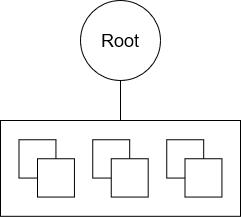
\includegraphics[width=.3\linewidth]{figures/SingleDirSystem.png}
                \caption{Esempio di Single Level Directory System}
                \label{fig:single-level-directory}
            \end{figure}

            \paragraph*{}

            L'approccio a livello unico offre alcuni vantaggi distinti. In primo luogo, la semplicità della struttura lo rende facile da implementare e utilizzare, poiché non sono necessari meccanismi complessi per navigare tra directory o sottodirectory. Inoltre, la localizzazione dei file è immediata, poiché tutto è contenuto all'interno di una singola cartella, rendendo inutile un sistema di ricerca avanzato.

            Tuttavia, questo modello ha limitazioni significative, soprattutto per applicazioni più complesse o ambienti che richiedono la gestione di un elevato numero di file.

            Per questo motivo, i sistemi a directory singola sono utilizzati principalmente in dispositivi embedded o sistemi con esigenze limitate, come fotocamere digitali o dispositivi elettronici di consumo basilari. In tali contesti, la semplicità e la leggerezza dell'architettura superano le necessità di una maggiore organizzazione.

        \subsection{Hierarchical Directory Systems}

            A differenza del modello a singolo livello, i sistemi a directory gerarchica sono progettati per rispondere alle esigenze dei moderni ambienti informatici, caratterizzati dalla gestione di grandi volumi di dati e file.

            
            In questo tipo di file system, è possibile creare una struttura organizzata composta da directory e sottodirectory. Questa struttura consente di suddividere i file in categorie o gruppi logici, favorendo una gestione più efficiente e un accesso più rapido alle informazioni.
            
            \paragraph*{}
            
            \begin{figure}
                \centering
                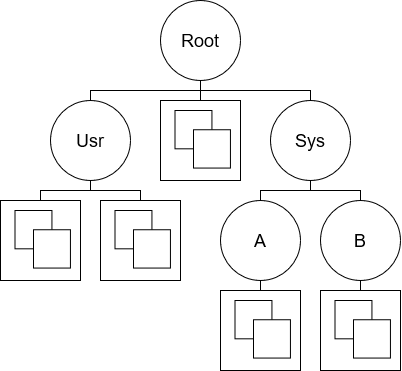
\includegraphics[width=.5\linewidth]{figures/MultipleDirSystem.png}
                \caption{Esempio di Hierarchical Directory System}
                \label{fig:hierarchical-directory}
            \end{figure}

            L'organizzazione gerarchica risulta particolarmente utile quando il sistema deve gestire elevate quantità di file. La possibilità di classificare i file in directory dedicate consente di mantenere ordine e chiarezza, riducendo la complessità che deriverebbe dall'avere tutto in un'unica directory.

            Un ulteriore vantaggio di questo approccio emerge nei contesti multiutente, dove più utenti condividono lo stesso file server. In questi casi, ogni utente può disporre di una directory root personale, che funge da punto di partenza per una gerarchia dedicata. Questa configurazione garantisce non solo la separazione dei dati tra gli utenti, ma anche un livello di personalizzazione che si adatta alle esigenze individuali.

            \paragraph*{}

            In conclusione, mentre i sistemi a livello singolo sono ideali per applicazioni semplici e specifiche, i sistemi gerarchici rappresentano una soluzione robusta e scalabile per ambienti complessi e moderni.

        \cite{tanenbaum2015modern}

    \section{Data Structures}

        Una struttura dati è un modo per memorizzare e organizzare i dati al fine di facilitare l'accesso e le modifiche.

        Sono elementi fondamentali nella progettazione e nell'implementazione dei file system, poiché determinano come i dati vengono organizzati, memorizzati e recuperati, influenzando direttamente l'efficienza e le prestazioni delle operazioni sui dati.

        Nessuna struttura dati singola è ottimale per tutti gli scopi, quindi è importante conoscere i punti di forza e le limitazioni delle diverse strutture.

        La scelta della struttura dati appropriata dipende da vari fattori, tra cui le esigenze specifiche del sistema, le prestazioni richieste e le limitazioni hardware.

        Tra le strutture dati più comuni utilizzate nei file system, si possono citare:

        \begin{itemize}
            \item Linked List: una sequenza di nodi collegati tra loro, in cui ogni nodo contiene un riferimento al nodo successivo.
            \begin{figure} [h]
                \centering
                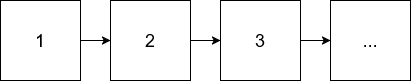
\includegraphics[width=.4\linewidth]{figures/LinkedList.png}
                \caption{Esempio di Linked List}
                \label{fig:linked-list}
            \end{figure}
            \item Array: una collezione di elementi disposti in una sequenza lineare, in cui ogni elemento è accessibile tramite un indice numerico.
            \begin{figure} [h]
                \centering
                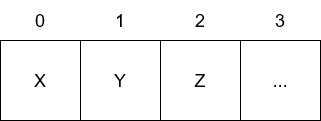
\includegraphics[width=.3\linewidth]{figures/Array.png}
                \caption{Esempio di Array}
                \label{fig:array}
            \end{figure}
            \item Tree: una struttura gerarchica composta da nodi collegati tra loro, in cui ogni nodo può avere uno o più nodi figli.
            \begin{figure} [h]
                \centering
                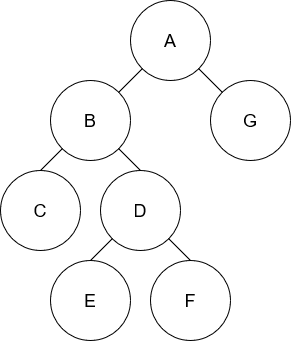
\includegraphics[width=.2\linewidth]{figures/Tree.png}
                \caption{Esempio di Tree}
                \label{fig:generic-tree}
            \end{figure}
            \item Hash Table: una struttura dati che associa chiavi a valori, consentendo un accesso rapido e diretto ai dati.
            \begin{figure} [h]
                \centering
                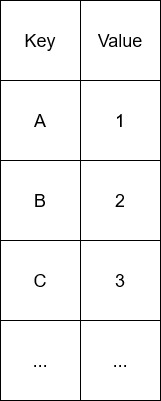
\includegraphics[width=.15\linewidth]{figures/HashTable.png}
I              \caption{Esempio di Hash Table}
                \label{fig:hash-table}
            \end{figure}
        \end{itemize}

        \cite{cormen2022introduction}

    \section{Strutture Dati Basate sui Tree}

        Le strutture dati come Linked List e Array sono strumenti potenti per rappresentare relazioni lineari, dove gli elementi sono disposti in una sequenza.Tuttavia, non tutte le relazioni nel mondo reale sono lineari.

        Molti problemi richiedono la rappresentazione di relazioni gerarchiche o ramificate, dove un elemento può essere connesso a più elementi in modo non sequenziale.

        \paragraph*{}

        Un Tree è una struttura dati non lineare composta da nodi collegati tra loro in modo gerarchico.

        Ogni albero ha un Nodo Radice denominato Root da cui partono uno o più Nodi denominati Figli, e ogni Figlio può a sua volta avere altri Figli, formando una struttura ramificata.

        \paragraph*{}

        In questo capitolo esploreremo le principali tipologie di alberi, le loro caratteristiche, i vantaggi e gli svantaggi.

        \subsection{Binary Trees}

            Un Binary Tree è la variante più basilare dei Tree in cui ogni nodo può avere al massimo due Figli, chiamati Figlio Sinistro e Figlio Destro, ed è rappresentato tramite tre attributi per nodo: `Key` (Il Valore), `Left` (Figlio Sinistro) e `Right` (Figlio Destro).

            Questa struttura è semplice, versatile e ampiamente utilizzata per realizzare strutture dati più avanzate.

            \paragraph*{}

            Un Binary Tree risulta essere semplice, efficiente e flessibile, ma può risultare inefficiente in caso di sbilanciamento e non è adatto a rappresentare relazioni con più di due figli.

        \subsection{Binary Search Trees}

            Un Binary Search Tree è un tipo di Binary Tree in cui ogni nodo rispetta un ordine: il valore del nodo è maggiore di tutti i valori nel suo sottoalbero sinistro e minore di tutti quelli nel sottoalbero destro.

            \paragraph*{}

            Questa struttura è utile per operazioni efficienti di ricerca, inserimento e cancellazione, e mantiene i nodi ordinati, semplificando operazioni come la ricerca del minimo o del massimo.

            \paragraph*{}

            Tuttavia, se l'albero non è bilanciato, può degenerare in una lista collegata perdendo così tutti i suoi benefici.

        \subsection{Balanced Trees}
            I Balanced Trees, come AVL e Red-Black, sono Binary Search Trees che mantengono l'altezza logaritmica rispetto al numero di nodi per garantire efficienza.

            \paragraph*{}

            Sia gli AVL che i Red-Black Trees utilizzano algoritmi e regole specifiche per mantenere l'equilibrio.

            \paragraph*{}

            Entrambi offrono prestazioni garantite come ricerca, inserimento e cancellazione in tempi brevi, rendendoli ideali per applicazioni che richiedono velocità e prevedibilità.

            Tuttavia, la gestione del bilanciamento richiede algoritmi più complessi rispetto ai BST standard, con un maggiore overhead computazionale dovuto alle operazioni di bilanciamento.

        \subsection{N-ary Trees}

            Un N-ary Tree è una generalizzazione dei Binary Trees in cui ogni nodo può avere fino a N Figli, con N come costante.

            \paragraph*{}

            Può essere rappresentato tramite array o liste di puntatori ai figli ed è utile per relazioni con un numero fisso di figli, come negli alberi di decisione nei giochi di scacchi.

            \paragraph*{}

            Il problema principale con gli N-ary Tree è la scelta del valore di N.

            Se il valore è troppo piccolo, le operazioni risultano efficienti, ma può verificarsi uno spreco di memoria quando molti nodi hanno meno di N figli, e la struttura risulta rigida per relazioni con un numero variabile di figli.

            Mentre se il valore è troppo grande, la struttura tende a diventare troppo simile ad una Linked List, con un aumento della complessità computazionale.

        \cite{cormen2022introduction}

    \section{B-Tree}

        Un B-Tree è un Balanced Search Tree progettato per mantenere i dati ordinati e permettere operazioni di ricerca, inserimento e cancellazione in tempo logaritmico.

        A differenza di altri Balanced Trees come i Red-Black Trees, i B-Tree sono ottimizzati per ridurre al minimo il numero di accessi al disco, rendendoli ideali per applicazioni che gestiscono grandi quantità di dati su dispositivi di memorizzazione secondaria.

        \paragraph*{}

        Indicando con \( n \) il numero massimo di Nodi Figli a cui un Nodo può puntare, un B-Tree ha le seguenti proprietà:

        \begin{itemize}
            \item Il numero massimo di Chiavi per Nodo è \( n - 1 \).
            \item Il Nodo Root è o un Nodo Foglia o un Nodo Interno con un numero di Figli compreso tra \( 2 \) e \( n \) e un numero di chiavi compreso tra \( 1 \) e \( n - 1 \).
            \item Tutti gli altri Nodi Interni hanno un numero di Figli compreso tra \( n / 2 \) e \( n \).
            \item Tutte le Foglie si trovano alla stessa profondità.
        \end{itemize}

        Queste proprietà garantiscono che il B-Tree rimanga bilanciato, mantenendo un'altezza relativamente bassa anche con un grande numero di elementi.

\chapter{Design and Implementation}

    \section{Analisi}

        Come precedentemente menzionato in \cref{sec:background}, la piattaforma IOtto rappresenta una soluzione IoT progettata per garantire il controllo completo degli impianti e dei macchinari ad essa connessi, ottimizzandone la manutenzione e la gestione energetica all'interno del contesto aziendale.

        \paragraph*{}

        Tra le numerose funzionalità offerte dal sistema, spiccano quelle relative al monitoraggio e all'analisi dei dati raccolti, operazioni che richiedono un elevato numero di accessi alla memoria fisica del sistema stesso.

        Queste funzionalità sono strettamente correlate alla scalabilità del sistema, che varia in base alle esigenze del cliente, con un numero di accessi alla memoria che può oscillare da poche centinaia a diverse decine di migliaia al giorno.

        \paragraph*{}

        Il sistema attuale, sebbene sia in grado di gestire volumi elevati di operazioni di lettura e scrittura, non risulta ottimizzato sotto diversi aspetti. Ad esempio, il formato utilizzato per la storicizzazione dei dati, denominato MessagePack, si rivela inefficiente in termini di consumo di risorse, specialmente quando si tratta di memorizzare dati di piccole dimensioni.

        \paragraph*{}

        Un ulteriore punto critico è rappresentato dal sistema di storicizzazione dei dati, basato su una struttura gerarchica tradizionale composta da cartelle e file. Questo approccio comporta tempi di ricerca, inserimento e rimozione che crescono in modo lineare, una caratteristica che, sebbene accettabile per un file system generico, risulta inadeguata per gestire il volume elevato di dati che il sistema potrebbe essere chiamato a gestire.

        \paragraph*{}

        Il software da sviluppare consiste in un prototipo che rappresenta una versione migliorata e ottimizzata dell'attuale file system. L'obiettivo del prototipo è introdurre ottimizzazioni che non alterino la struttura esistente, con particolare attenzione ai processi di gestione e storicizzazione dei dati.

        \subsection{Requisiti Funzionali}

            \begin{itemize}
                \item Il sistema deve supportare un formato di serializzazione che, rispetto a soluzioni esistenti come MessagePack, sia ottimizzato per la gestione di dati di piccole dimensioni.
                \item È prevista l’implementazione di un sistema di indicizzazione il cui obiettivo è ridurre la complessità computazionale delle varie operazioni, passando da un algoritmo con complessità lineare a uno con complessità logaritmica.
                \item Il progetto prevede interventi strutturali finalizzati a migliore delle operazioni di ricerca, inserimento e rimozione, migliorando l’efficienza complessiva del sistema e riducendo i tempi di risposta alle richieste.
                \item Il sistema deve essere progettato per gestire un carico variabile di operazioni. Tale requisito implica che il sistema debba garantire performance costanti, attraverso una scalabilità sia verticale che orizzontale.
                \item Devono essere implementati meccanismi affidabili per il backup e il ripristino dei dati. Questi meccanismi devono assicurare l’integrità e la disponibilità delle informazioni, minimizzando il rischio di perdita di dati e garantendo un rapido recupero in caso di malfunzionamenti o incidenti.
                \item Il prototipo sviluppato dovrà integrarsi la struttura attualmente in uso. Tale integrazione deve avvenire senza introdurre impatti negativi sull’architettura esistente, consentendo una transizione fluida e minimizzando eventuali disservizi.
            \end{itemize}

        \subsection{Requisiti Non Funzionali}

            \begin{itemize}
                \item Per garantire una manutenzione efficace e una facile estendibilità del sistema, è necessario implementare una documentazione esaustiva.
                \item Viene richiesta una struttura modulare dell’architettura, che consenta di aggiornare o sostituire singoli componenti senza dover riprogettare l’intero sistema.
                \item L’interoperabilità tra diverse piattaforme è un requisito fondamentale per garantire un’ampia adozione del sistema. La compatibilità con ambienti Linux e Windows, unitamente al supporto per architetture hardware sia x86 che ARM, assicura che il software possa essere implementato in contesti eterogenei.
                \item Una caratteristica essenziale dell’architettura è la capacità di integrare dinamicamente nuovi nodi di storage in un ambiente di produzione, senza interrompere il servizio.
                \item Il sistema deve prevedere un livello di configurabilità dei vari parametri, permettendo agli amministratori di ottimizzare il comportamento in funzione delle specifiche esigenze applicative e dei requisiti di performance.
            \end{itemize}

    \section{Design}

        L'intera fase di design è avvenuta attraverso un processo iterativo, che ha coinvolto me e il team manager, con l'obiettivo di garantire che il prototipo rispondesse in modo efficace ai requisiti identificati.

        \paragraph*{}

        Dopo alcune ricerche preliminari, abbiamo deciso di utilizzare un B-Tree come struttura dati principale per il prototipo, poiché, sulla base di un'attenta valutazione delle prestazioni attese in scenari reali, esso si è dimostrato particolarmente adatto a gestire grandi volumi di dati garantendo elevate prestazioni.

        Le caratteristiche che hanno reso questa struttura ottimale includono:

        \begin{itemize}
            \item \textbf{Bilanciamento Automatico}: garantisce complessità O(log n) per ricerche, inserimenti e cancellazioni, anche con dataset in crescita dinamica.
            \item \textbf{Efficienza nell’I/O su disco}: la struttura ad albero, con nodi di grado elevato, riduce il numero di accessi al disco, cruciale per dataset di dimensioni superiori alla RAM disponibile.
            \item \textbf{Scalabilità}: capacità di gestire milioni di record senza perdita prestazionale.
        \end{itemize}

        Un confronto con alternative come i Binary Trees (Soggetti al problema dello Sbilanciamento) o alle Hash Table (Inefficienti in operazioni di Range Query) ha confermato la superiorità del B-Tree nel contesto del progetto.

        Inoltre, l’uso del B-Tree è supportato da letteratura consolidata in ambito di Database Systems, rafforzandone la validità come scelta progettuale, come ad esempio \cite{mostafa2020case}.

        \paragraph*{}

        Per ottimizzare l’uso della memoria e ridurre gli sprechi, è stato implementato un sistema customizzato di serializzazione/deserializzazione binaria, in sostituzione di MessagePack.

        Le motivazioni includono:
        \begin{itemize}
            \item \textbf{Controllo Granulare}: la serializzazione manuale ha permesso di definire formati compatti per ogni dato, eliminando metadati superflui, come le Chiavi JSON, e utilizzando tipi a lunghezza fissa dove possibile, ad esempio interi a 32 bit invece di valori variabili.
            \item \textbf{Riduzione dell’Overhead}: rispetto a MessagePack, il formato custom riduce la dimensione dei dati serializzati, soprattutto grazie all’assenza di header descrittivi.
            \item \textbf{Flessibilità nelle modifiche}: la struttura binaria è progettata per essere estendibile senza impattare sulla backward compatibility, ad esempio riservando bit per flag futuri.
        \end{itemize}




        \subsection{Componenti}

            \begin{itemize}
                \item \textbf{Data Manager}: Questo componente si occupa della gestione dei dati, fornendo funzionalità di lettura, scrittura, ricerca e rimozione. Il Data Manager è progettato per garantire prestazioni elevate e un accesso efficiente ai dati, riducendo al minimo i tempi di ris
            \end{itemize}

%%%%% \lstinputlisting[float,language=Java,label={lst:random-code}]{listings/HelloWorld.java}

%----------------------------------------------------------------------------------------
% BIBLIOGRAPHY
%----------------------------------------------------------------------------------------

\backmatter

\nocite{*} % Remove this as soon as you have the first citation

\bibliographystyle{alpha}
\bibliography{bibliography}

\begin{acknowledgements} % this is optional
Optional. Max 1 page.
\end{acknowledgements}

\end{document}
